\documentclass{article}
\usepackage[T5]{fontenc}
\usepackage[utf8]{inputenc}
\usepackage{listings}
\usepackage{tabularx}
\usepackage{geometry}
\usepackage[numbers]{natbib}
 \geometry{
 a4paper,
 total={170mm,257mm},
 left=20mm,
 top=20mm,
 }
\usepackage{graphicx}
\usepackage{hyperref}
\renewcommand*\contentsname{Mục lục}
\renewcommand{\bibsection}{\textit{\textbf{Tài liệu tham khảo}}}
\begin{document} 

\begin{titlepage}

    \centering % Centre everything on the title page
    {Trường Đại học Khoa học Tự nhiên \\ Đại học Quốc gia Thành phố Hồ Chí Minh\\}
    
    \vspace*{4\baselineskip} % White space at the top of the page
	
    {\LARGE CƠ SỞ TRÍ TUỆ NHÂN TẠO\\} % Title
    \vspace*{5\baselineskip}
    
    \rule{\textwidth}{0.4pt}
    \vspace*{-\baselineskip}
    \vspace*{2pt} % Thick horizontal rule
	
    \vspace*{0.75\baselineskip} % Whitespace above the title

    {\Huge CÁC THUẬT TOÁN \\ TÌM KIẾM \\ TRÊN ĐỒ THỊ \\}
	
    \vspace{0.75\baselineskip} % Whitespace below the title
	
    \rule{\textwidth}{0.4pt}
	
    \vspace{1\baselineskip} 

    {\# Đồ án 1\\}
        
    \vspace{2\baselineskip}
    
    {\large Sinh viên: \Large Phan Huy Trường\\}
    \vspace{0.75\baselineskip}
    {\large MSSV: \Large 20120231\\}
    \vspace{0.75\baselineskip}
    {\Large Lớp 20\_22}
	
    \vspace{0.5\baselineskip} % Whitespace below the editor list
	
	
    \vfill 
	
	
    10/2022 % Publication year
	
    {\large Tp. Hồ Chí Minh} % Publisher

\end{titlepage}

%----------------------------------------------------------------------------------------
\tableofcontents
\newpage
\section{Tự đánh giá}
\begin{table}[ht]
\centering
    \begin{tabular}{|c|l|c|}
    \hline
    \textbf{STT} & \multicolumn{1}{c|}{\textbf{Tiêu chí}} & \textbf{Đánh giá}     \\ \hline
    1 & Tìm hiểu và trình bày được các thuật toán   & 10    \\ \hline
    2 & So sánh các thuật toán với nhau        & 10                    \\ \hline
    3 & \begin{tabular}[c]{@{}l@{}}Cài đặt được các thuật toán DFS, BFS, UCS, AStar.\\ Mô tả và nhận xét được các thuật toán trên\end{tabular} & 10    \\ \hline
    5 & Tìm hiểu thêm các thuật toán ngoài yêu cầu  & 8   \\ \hline
    \multicolumn{2}{|c|}{\textit{\textbf{Trung bình}}}  & \textit{\textbf{9.5}} \\ \hline
    \end{tabular}
\end{table}
\newpage
\section{Báo cáo về các thuật toán tìm kiếm}

%-------------------------------------------------

\subsection{Thuật toán Depth-First-Search (DFS)}
\subsubsection{Ý tưởng chung}
\begin{itemize}
    \item Phát triển các nút chưa xét theo chiều sâu – Các nút 
được xét theo thứ tự độ sâu giảm dần
    \item Thuật toán khởi đầu tại một đỉnh và tiếp tục tìm kiếm theo hướng mở các nút ở sâu nhất trước cho đến khi tìm được đích hoặc nút đó không còn đi tiếp được nữa
    \item Khi nút đó không còn có thể mở sâu thêm, thuật toán sẽ quay lui dựa theo đường đi đã mở trước đó để tìm nút có thể mở
\end{itemize}

\subsubsection{Mã giả}
\begin{verbatim}
    # Sử dụng ngăn xếp LIFO (các nút mới được lưu vào đầu open_set)
    
    DFS(graph, start){
        Stack open_set = {start};
        Array closed_set = {}
        while (open_set is not empty)
        {
            s = open_set.getFirst()
            closed_set.append(s)    
            if(graph.is_Goal(s)){
                return path()
            }
            for each neighbor of s{
                if (neighbor not in closed_set ){ 
                    open_set.append(neighbor)
                }   
            }
        } 
        return ('No Solution')
    }
\end{verbatim}

\subsubsection{Đánh giá về thuật toán}
\begin{quote}
    b: số nhánh tối đa\\
    m: chiều sâu tối đa
\end{quote}
\begin{itemize}
    \item \textbf{Độ phức tạp thời gian:} $O(b^m)$
    \item \textbf{Độ phức tạp không gian:} $O(bm)$ nếu không gian trạng thái là hữu hạn
    \item \textbf{Tính hoàn chỉnh:} Có nếu không gian hữu hạn
    \item \textbf{Tính tối ưu:} Không, DFS sẽ luôn cho ra lời giải phải nhất cho dù lời giải đó không là tối ưu
\end{itemize}
\subsubsection{Ví dụ}
    \centerline{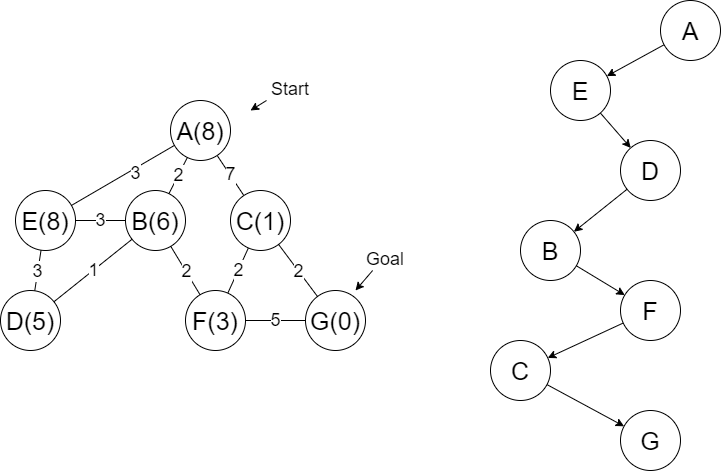
\includegraphics[width=4in, height=2.5in]{image/dfs.png}}
    \vspace{2\baselineskip}

%--------------------------------------------------------

\subsection{Thuật toán Breadth-First-Search (BFS)}
\subsubsection{Ý tưởng chung}
\begin{itemize}
    \item Phát triển các nút chưa xét theo thứ tự tăng dần - Các nút được xét theo thứ tự độ sâu tăng dần
    \item Thuật toán khởi đầu tại một đỉnh và duyệt hết các nút lân cận trước khi duyệt các lận cận của đỉnh tiếp theo kề với đỉnh gốc
\end{itemize}

\subsubsection{Mã giả}

\begin{verbatim}
    # Sử dụng hàng đợi FIFO (các nút mới được lưu vào cuối open_set)
    
    BFS(graph, start){
        Queue open_set = {start};
        Array closed_set = {}
        while (open_set is not empty)
        {
            s = open_set.getFirst()
            closed_set.append(s)    
            if(graph.is_Goal(s)){
                return path()
            }
            for each neighbor of s{
                if (neighbor not in closed_set and not in open_set){ 
                    open_set.append(neighbor)
                }   
            }
        } 
        return ('No Solution')
    }
\end{verbatim}

\subsubsection{Đánh giá về thuật toán}
\begin{quote}
    b: số nhánh tối đa
    d: chiều sâu của lời giải nông nhất
\end{quote}
\begin{itemize}
    \item \textbf{Độ phức tạp thời gian:} $1 + b + b^2 + b^3 + \dots + b^d = O(b^d)$
    \item \textbf{Độ phức tạp không gian:} $O(b^d-1)$ cho tập mở và $O(b^d)$ cho biên
    \item \textbf{Tính hoàn chỉnh:} Thuật toán có tính hoàn chỉnh nếu b là hữu hạn và không gian trạng thái có lời giải và hữu hạn 
    \item \textbf{Tính tối ưu:} Thuật toán có tính tối ưu nếu chi phí là như nhau ở mỗi bước
\end{itemize}

\subsubsection{Ví dụ}
    \centerline{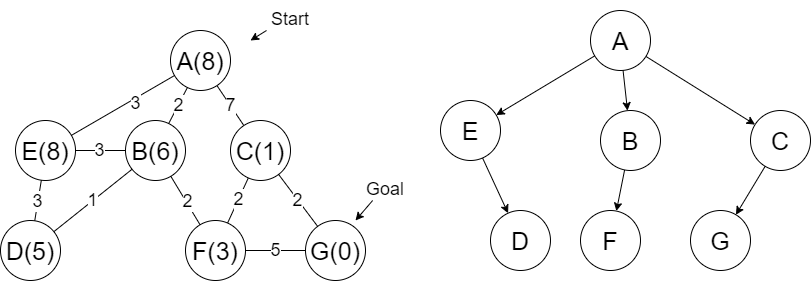
\includegraphics[width=5in, height=2.5in]{image/bfs.png}}
    \vspace{2\baselineskip}
%-------------------UCS--------------------%
\subsection{Thuật toán UCS}
\subsubsection{Ý tưởng chung}
\begin{itemize}
    \item Mở các nút chưa xét dựa trên chi phí đường đi thấp nhất - Các nút được mở với thứ tự chi phí tăng dần
    \item Thuật toán dựa vào hàm đánh giá $f(n) = g(n)$ để tìm kiếm đường đi. Trong đó g(n) là chi phí thực tế đi đến nút đang xét
    \item Thuật toán sử dụng cấu trúc hàng đợi ưu tiên. Thuật toán bắt đầu nút gốc và duyệt các nút tiếp theo dựa trên chi phi đi từ nút đang xét đến đỉnh gốc.
\end{itemize}

\subsubsection{Mã giả}
\begin{verbatim}
    UCS(graph, start){
        PriorityQueue open_set = {start};
        Array closed_set = {}
        while (open_set is not empty)
        {
            s = open_set.GET_LOWEST_COST_NODE()
            closed_set.append(s)  
            if(graph.is_Goal(s)){
                return path()
            }
            for each neighbor of s{
                if (neighbor not in closed_set ){ 
                    open_set.append(neighbor)
                }   
            }
        } 
        return ('No Solution')
    }
    
\end{verbatim}
\subsubsection{Đánh giá về thuật toán}
\begin{itemize}
    \item \textbf{Độ phức tạp thời gian:} Phụ thuộc vào tổng số các nút có chi phí $\leq$ chi phí của lời giải tối ưu\\
    Độ phức tạp thời gian: $O(b^{1 + \lfloor C^*/\epsilon\rfloor})$\\
    Trong đó:\\
    $\epsilon$: chi phí di chuyển thấp nhất\\
    $C^*$: chi phí của lời giải tối ưu
    \item \textbf{Độ phức tạp không gian:} $O(b^{1 + \lfloor C^*/\epsilon\rfloor})$\\
    $O(b^{1 + \lfloor C^*/\epsilon\rfloor})$ có thể lớn hơn nhiều so với $O(b^d)$ bởi vì thuật toán ưu tiên mở rộng các nhánh lớn với chi phí thấp trước khi mở những nút nằm ở xa hơn với chi phí cao. Khi chi phí di chuyển là như nhau ở các bước thì độ phức tạp của UCS có thể tương đương với BFS $O(b^d)$
    \item \textbf{Tính hoàn chỉnh:} Có nếu không gian, số nhánh hữu hạn và chi phí di chuyển thấp nhất $\epsilon > 0$
    \item \textbf{Tính tối ưu:} Có nếu không tồn tại chi phí < 0
\end{itemize}
\subsubsection{Ví dụ}
    \centerline{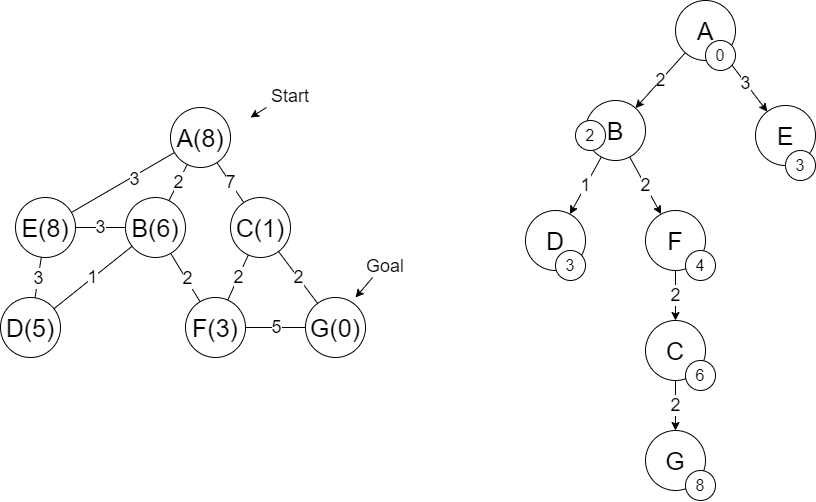
\includegraphics[width=4in, height=2.5in]{image/ucs.png}}
    \vspace{2\baselineskip}
\subsection{Thuật toán AStar}
\subsubsection{Ý tưởng}
\begin{itemize}
    \item Kết hợp giữa Uniform-Cost-Search và Greedy Best-First-Search. 
    \item A* Search sử dụng hàm đánh giá tích hợp heuristic vào quá trình tìm kiếm, tránh các đường đi có chi phí lớn. Hàm đánh giá của A* được xây dưng như sau:\\
    $g(n)$: chi phí từ nút gốc đến nút hiên tại n\\
    $h(n)$: chi phí ước tính từ nút hiện tại n đến nút gốc \\
    $f(n) = g(n) + h(n)$
\end{itemize}
\subsubsection{Mã giả}
\begin{verbatim}
    AStar(graph, start){
        open_set[start] = 0
        List closed_set = {}
        List cost = []
        g_cost[start] = 0
        f_cost[start] = heuristic_cost between start and goal
        while (open_set is not empty)
        {
            current = node in open_set have lowest f_cost
            closed_set.append(s)  
            remove current from open_set
            if(current is goal){
                return path()
            }
            for each neighbor of current{
                if(neighbor in closed_set)
                    continue
                tentative_g_cost = g_cost[current] + distance_between(current, neighbor)
                if neighbor not in openset or tentative_g_cost < g_cost[neighbor] 
                    g_score[neighbor] := tentative_g_score
                    f_score[neighbor] := g_score[neighbor] + heuristic_cost(neighbor,goal)
                    if neighbor not in openset
                        add neighbor to openset 
            }
        } 
        return ('No Solution')
    }
\end{verbatim}
\subsubsection{Đánh giá}
\begin{itemize}
    \item \textbf{Độ phức tạp thời gian:} Phụ thuộc vào hàm heuristic. Trong trường hợp tệ nhất, số nút được mở rộng theo cấp số mũ, độ phức tạp lên tới $O(b^d)$ \vspace{2pt}\\
     Độ phức tạp thời gian là một hàm đa thức khi không gian tìm kiếm là một cây, có một trạng thái đích và hàm heuristic được chọn thỏa mãn điều kiên:$| h(n) - h*(n) | = O(log h*(n) )$ (Trong đó $h*(n)$ là một heuristic tối ưu, chi phí chính xác từ nút đó đến đích)
    \item \textbf{Độ phức tạp không gian:} Tương tự với những thuật toán khác $O(b^d)$ 
    \item \textbf{Tính hoàn chỉnh: }Thuật toán là hoàn chỉnh nếu chi phi di chuyển thấp nhất $\epsilon > 0$ và không gian trạng thái là hữu hạn hoặc tồn tại nghiệm
    \item \textbf{Tính tối ưu: }Thuật toán có tính tối ưu nếu heuristic hợp lý và nhất quán
    
\end{itemize}

\subsubsection{Ví dụ}
    \centerline{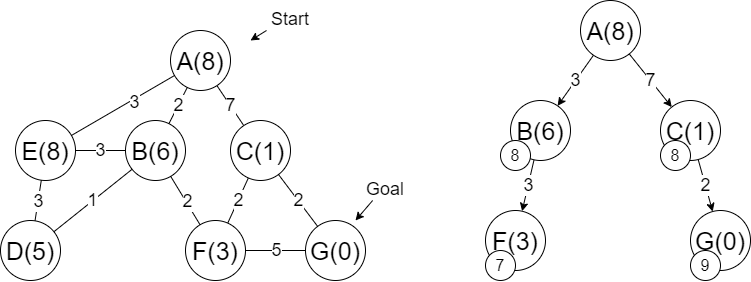
\includegraphics[width=5in, height=2.5in]{image/astar.png}}
    \vspace{2\baselineskip}
\section{So sánh sự khác biệt giữa các thuật toán tìm kiếm}
\subsection{So sánh sự khác biệt giữa UCS, Greedy, A*}
\hspace{0.5in} Ý tưởng chung của các thuật toán này đều sử dụng hàm đánh giá $f(n)$ trong việc tìm kiếm đường đi, tuy nhiên các hàm đánh giá là khác nhau ở từng thuật toán khiến cho chi phí tìm kiếm là khác nhau ở các thuật toán.\\
\begin{table}[h!]
    \centering
    
    \begin{tabular}{ |p{2.5cm}|p{3cm}|p{3cm}|p{3cm}|  }\hline
    &   \textbf{UCS}    &  \textbf{Greedy}  &   \textbf{AStar}\\  
    \hline
    Hàm đánh giá&$f(n) = g(n)$&$f(n) = h(n)$&$f(n) = g(n) + h(n)$\\ \hline
    Chiến lược tìm kiếm&Tìm kiếm mù&Tìm kiếm có định hướng&Tìm kiếm có định hướng\\ \hline
    Tính hoàn chỉnh& Có&Không&Có \\ \hline
    Tính tối ưu&Có& Không& Có \\ \hline
    \multicolumn{4}{c}{\footnotesize $g(n):$ chi phí thực tế từ nút gốc đến nút n}\\
    \multicolumn{4}{c}{\footnotesize $h(n):$ hàm heuristic ước tính chi phí đến đích}\\
    \end{tabular}
\end{table}

\hspace{0.5in} Greedy Best-First-Search luôn cố gắng tìm những nút gần đích nhất có thể dựa theo hàm heuristic, do đó luôn tồn tại rủi ro thuật toán sẽ không tìm ra đường đi hoặc đường đi là không tối ưu. Trong khi đó A* là sự kết hợp giữa Greedy BFS và UCS do đó thuật toán đảm bảo tìm được đường đi tối ưu nếu heuristic là hợp lý và nhất quán. Khi $h(n) = 0$ A* sẽ là UCS và khi $g(n) = 0$A* sẽ là Greedy BFS
\subsection{So sánh sự khác biệt giữa UCS và Dijkstra}
\hspace{0.5in} Nhìn chung thuật toán Dijkstra và UCS là tương tự nhau về ý tưởng chung. Tuy nhiên cả hai có những điểm khác biệt như sau:
\begin{itemize}
    \item Thuật toán Dijkstra tìm kiếm đường đi ngắn nhất từ nút gốc cho đến mọi nút khác trong đồ thị. Trong khi đó UCS chú trọng vào việc tìm kiếm đường đi ngắn nhất đến nút đích hơn là tìm kiếm đường đi ngắn nhất đến mọi nút trong đồ thị
    \item Đối với UCS, thuật toán sẽ dừng lại bất cứ khi nào nút đích được tìm thấy. Đối với Dijkstra, thuật toán chỉ dừng lại khi tất cả mọi đỉnh trong đồ thị đã được duyệt qua.
    \item Do đó UCS tốn ít không gian lưu trữ và thời gian hơn Dijkstra vốn duyệt và lưu hết tất cả các nút
\end{itemize}


%-----------------------------------------------%
\section{Các thuật toán khác}

%------------------------------------------------
\subsection{Thuật toán Greedy Best-First-Search}
\subsubsection{Ý tưởng chung}
\begin{itemize}
    \item Cũng giống như các chiến lược tìm kiếm có định hướng khác, Greed BFS sử dụng hàm đánh giá $f(n) = h(n)$ để xác định nút tiếp theo được mở. Trong đó $h(n)$ là hàm heuristic thể hiện chi phí ước tính đến nút gốc.
    \item Theo đó, thuật toán chú trọng vào việc mở các nút có giá trị heuristic thấp nhất, nghĩa là các nút ở gần nút đích  nhất
\end{itemize}

\subsubsection{Mã giả}

\begin{verbatim}
    # Tương tự như mã giả của thuật toán AStar, chí khác ở chỗ không còn tồn tại hàm đánh giá hiện tại không có sự xuất hiện của $g(n)$
    
    Greedy(graph, start){
        open_set = start 
        List closed_set = {}
        f_cost[start] = heuristic_cost(start,goal)
        while (open_set is not empty)
        {
            current = node in open_set have lowest f_cost
            closed_set.append(s)  
            remove current from open_set
            if(current is goal){
                return path()
            }
            for each neighbor of current{
                if(neighbor in closed_set)
                    continue
                tentative_f_cost = heuristic_cost(neighbor,goal)
                if neighbor not in openset or tentative_f_cost < f_cost[neighbor]
                    f_cost[neighbor] = tentative_f_cost
                    if neighbor not in openset
                        add neighbor to openset 
            }
        } 
        return ('No Solution')
    }
\end{verbatim}

\subsubsection{Đánh giá về thuật toán}
\begin{itemize}
    \item \textbf{Độ phức tạp thời gian:} Trong trường hợp tệ nhất, độ phức tạp thời gian của Greedy BFS là tương tự với DFS $(O(b^m)$. Tuy nhiên độ phức tạp thời gian của Greedy có thể cải thiện nếu hàm heuristic là tốt
    \item \textbf{Độ phức tạp không gian:} $O(b^m)$ 
    \item \textbf{Tính hoàn chỉnh:} Không
    \item \textbf{Tính tối ưu:} Không
\end{itemize}

\subsubsection{Ví dụ}
    \centerline{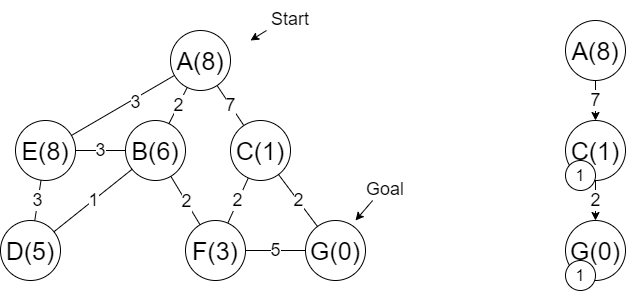
\includegraphics[width=4in, height=2.5in]{image/greedy.png}}
    \vspace{2\baselineskip}
%---------------------------------------------------
\subsection{Thuật toán Dijkstra}
\subsubsection{Ý tưởng chung}
\begin{itemize}
    \item Thuật toán tìm đường đi ngắn nhất từ nút khởi đầu đến các nút còn lại trong đồ thị
    \item Theo đó, thuật toán mở lần lượt các nút gần đích nhất và chỉ dừng lại khi tất cả các nút đã được mở
\end{itemize}

\subsubsection{Mã giả}

\begin{verbatim}
    Dijkstra(graph, start){
        closed_set = []
        distance = [1e7] * graph.size()
        distance[start] = 0
        for i in range(graph.size()){
            current = distance.minDistance()
            closed_set.append(current)
            for each neighbor of current{
                tentative_distance = distance[current] + distance_between(neighbor, current)
                if(neighbor not in closed_set and 
                distance[neighbor] > tentative_distance
                    distance[neighbor] = tentative_distance
            }
        }
    }
    
\end{verbatim}
\subsubsection{Đánh giá về thuật toán}
\begin{quote}
    V: số cạnh \hspace{0.5in}
    E: số đỉnh 
\end{quote}
\begin{itemize}
    \item \textbf{Độ phức tạp thời gian:} $O(V^2)$ nếu sử dụng ma trận kề và $O((V+E)logV$ nếu sử dụng danh sách kề
    \item \textbf{Độ phức tạp không gian:} $O(V+E)$ 
    \item \textbf{Tính hoàn chỉnh:} Tương tự UCS
    \item \textbf{Tính tối ưu:} Tương tự UCS
\end{itemize}

\subsubsection{Ví dụ}
    \centerline{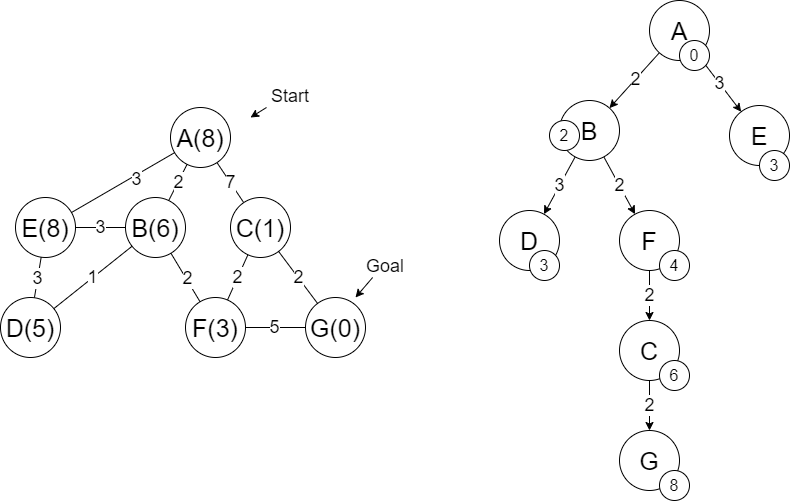
\includegraphics[width=4in, height=2.5in]{image/dijkstra.png}}
    \vspace{2\baselineskip}
    
\section{Cài đặt thuật toán}
\subsection{Thuật toán DFS}
    \centerline{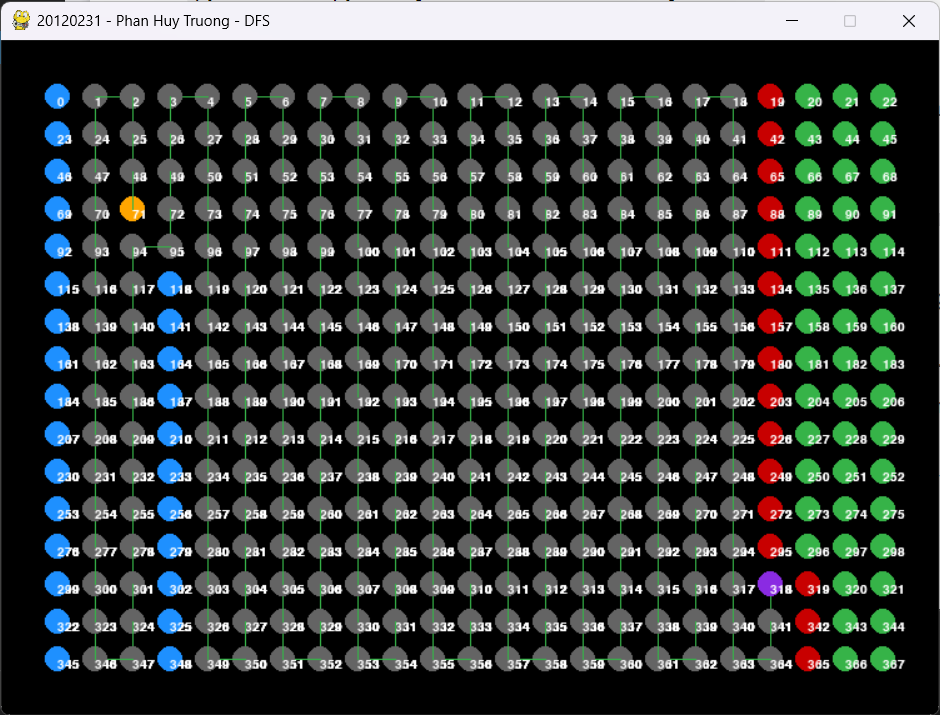
\includegraphics[width=4.5in, height=3in]{image/dfs_stimulation.png}}
    \textbf{Mô tả: }
    \begin{itemize}
        \item Khi khởi chạy thuật toán DFS tiến hành duyệt đồ thị theo chiều sâu tối đa trước khi bắt buộc phải quay lui.
        \item Trong quá trình thực hiện, thuật toán lưu vào đầu ngăn xếp open\_các nút được tìm thấy và đưa vào danh sách closed\_set các nút đã mở qua
        \item Đồng thời trong quá trình đó, thuật toán cũng lưu lại cha của những nút tìm thấy, nhầm thuận tiện cho việc vẽ lại đường đi tìm thấy
    \end{itemize}
    \textbf{Nhận xét: }
    \begin{itemize}
        \item Có thể thấy đường đi được tìm thấy sau khi khởi chạy là một đường đi không tối ưu khi đường đi bao gồm gần như tất cả các nút được duyệt.
        \item Thuật toán không quan tâm đến chi phỉ đường đi và khởi chạy theo tư duy vét cạn, do đó thuật toán tốn nhiều thời gian để hoàn thành.
    \end{itemize}
    
    \vspace{2\baselineskip}
\subsection{Thuật toán BFS}
    \centerline{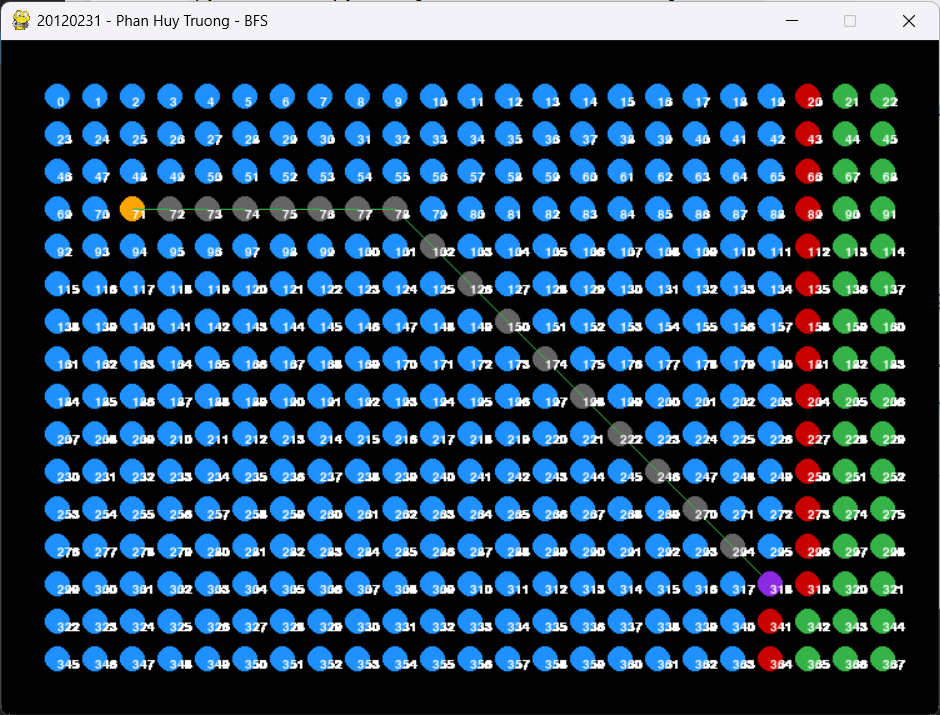
\includegraphics[width=4.5in, height=3in]{image/bfs_stimulation.png}}
    \vspace{2\baselineskip}
    \textbf{Mô tả: }
    \begin{itemize}
        \item Khi khởi chạy thuật toán tiến hành mở các nút ở bậc thấp trước khi mở các nút ở bậc cao hơn
        \item Trong quá trình thực hiện, thuật toán lưu các nút được tìm thấy vào hàng đợi open\_set và đưa vào danh sách closed\_set các nút đã được mở qua.
        \item Đồng thời trong quá trình đó, chương trình cũng tiến hành lưu lại những nút cha để tiện cho việc vẽ lại đường đi
    \end{itemize}
    \textbf{Nhận xét: }
    \begin{itemize}
        \item Thuật toán luôn trả về đường đi đi qua ít cạnh nhất 
        \item Thuật toán không quan tâm đến chi phỉ đường đi và khởi chạy theo tư duy vét cạn. Do đó thuật toán tồn nhiều thời gian để khởi chạy.
        \item Thuật toán cần nhiều bộ nhớ để lưu trữ hơn DFS
    \end{itemize}
    
\subsection{Thuật toán UCS}
    \centerline{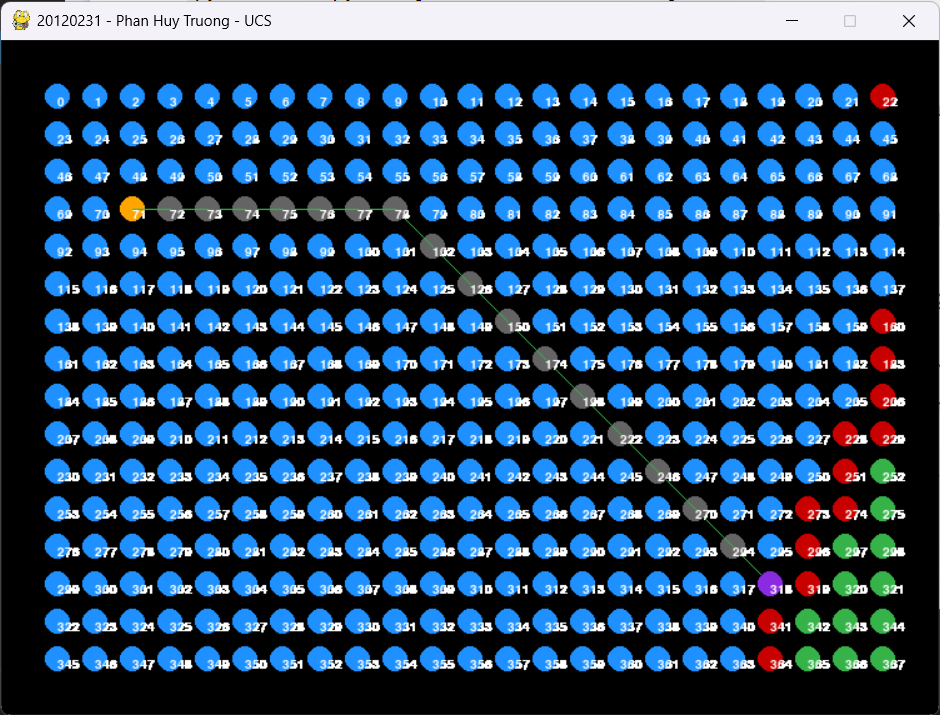
\includegraphics[width=4.5in, height=3in]{image/ucs_stimulation.png}}
    \vspace{2\baselineskip}
    \begin{itemize}
        \item Khi khởi chạy thuật toán tiến hành mở các nút ở gần nút gốc nhất
        \item Trong quá trình thực hiện, thuật toán lưu lại các nút được tìm thấy vào open\_set nếu chưa tồn tại hoặc thay đổi giá trị chi phí từ nút bắt đầu đến nút đang xét nếu chi phí là thấp hơn chi phí của nút đó được lưu trong open\_set và không thay đổi chi phí nếu chi phí tính được là cao hơn. Thuật toán cũng đưa vào danh sách closed\_set các nút đã được mở qua. Các nút mới được mở ở mỗi lần lặp lại là các nút có chi phí thấp nhất.
        \item Đồng thời trong quá trình đó, chương trình cũng tiến hành lưu lại những nút cha để tiện cho việc vẽ lại đường đi
    \end{itemize}
    \textbf{Nhận xét: }
    \begin{itemize}
        \item Thuật toán luôn trả về đường đi đi ngắn nhất tồn tại
        \item Thuật toán luôn quan tâm đến chi phí đường đi đến các nút. 
        \item Trong một số trường hợp, độ phức tạp của thuật toán lớn hơn cả độ phức tạp của BFS
    \end{itemize}
\subsection{Thuật toán A*}
    \centerline{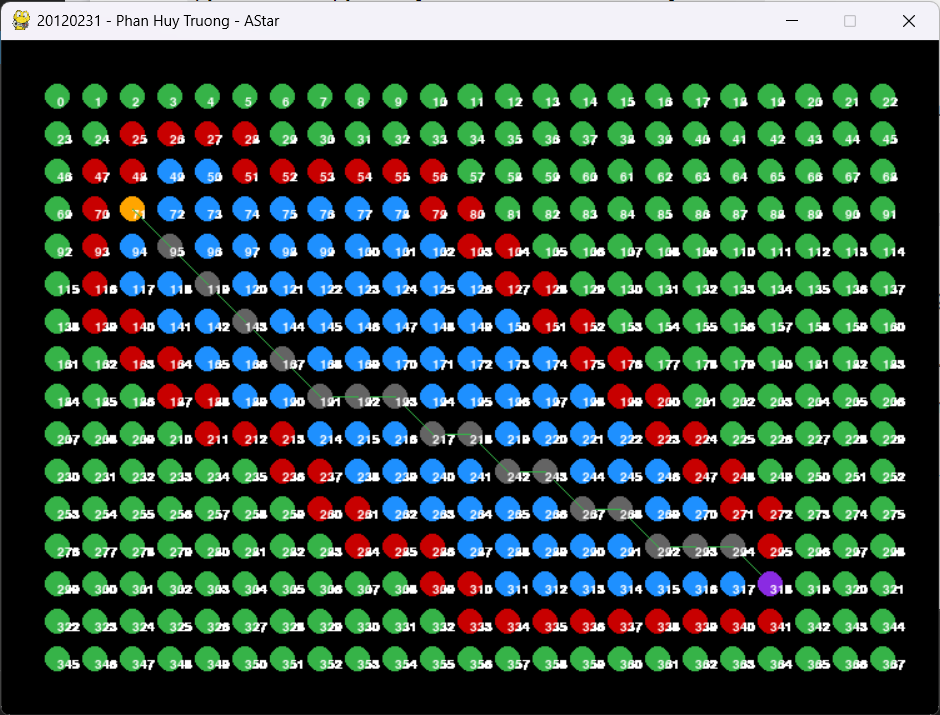
\includegraphics[width=4.5in, height=3in]{image/astar_stimulation.png}}
    \vspace{2\baselineskip}
    \begin{itemize}
        \item Thuật toán dựa vào hàm đánh giá $f(n) = g(n) + h(n)$ để tìm được đường đi. Trong đó $g(n)$ là chi phi từ nút bắt đầu đi đến nút hiện tại và $h(n)$ là một hàm heuristic ước tính chi phí. Hàm heuristic $h(n)$ được chọn ở đây là khoảng cách euclid từ nút đang xét cho đến nút đích. 
        \item Trong quá trình thực hiện, thuật toán lưu các nút được tìm thấy vào open\_set và đưa vào danh sách closed\_set các nút đã được mở qua đối với các nút chưa tồn tại trong open\_set hoặc thay đổi chi phí đánh giá $f(n)$ nếu chí phí đánh giá được là thấp hơn. Các nút mới được mở ở mỗi lần lặp lại là nút có chi phí đánh giá bởi hàm $f(n)$ thấp nhất
        \item Đồng thời trong quá trình đó, chương trình cũng tiến hành lưu lại những nút cha để tiện cho việc vẽ lại đường đi
    \end{itemize}
    \textbf{Nhận xét: }
    \begin{itemize}
        \item Thuật toán dựa vào hàm đánh giá $f(n)$ phụ thuộc vào 2 yếu tố chi phí thực tế và chi phí ước tính. Do đó A* là một giải thuật linh động, tổng quát, nhanh chóng tìm ra lời giải dưới sự định hướng của heuristic. 
        \item Thuật toán quan tâm đến chi phỉ đường đi.
        \item Tuy nhiên A* cần nhiều bộ nhớ để lữu trữ lại không gian trạng thái đã đi quá với độ phức tạp về mặt không gian là cấp số mũ
    \end{itemize}
\subsection{Thuật toán Greedy Best-First-Search}
    \centerline{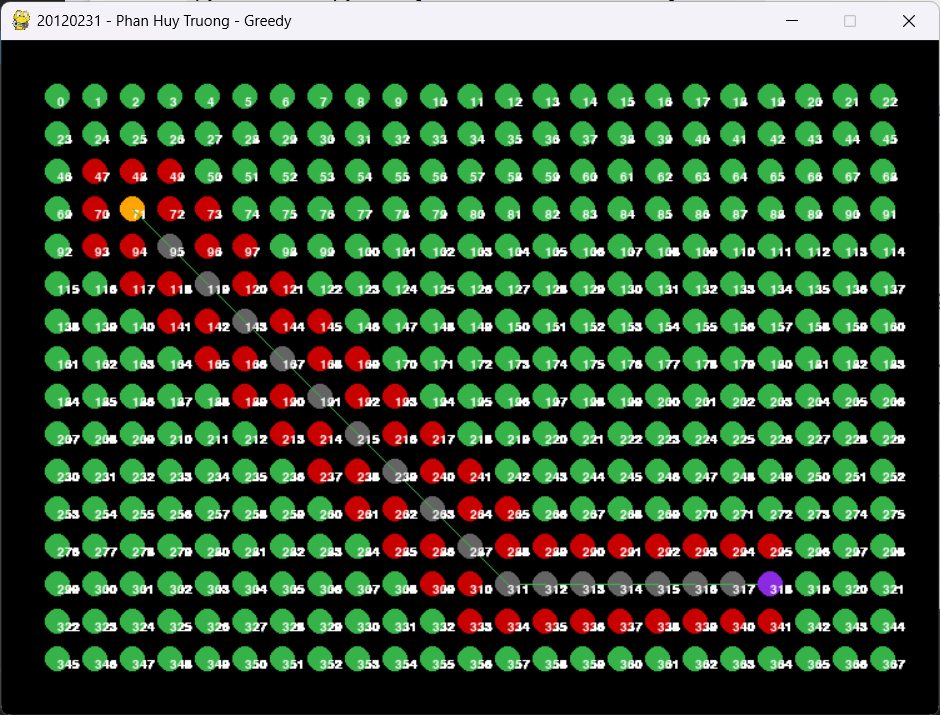
\includegraphics[width=4.5in, height=3in]{image/greedy_stimulation.png}}
    \vspace{2\baselineskip}
    \begin{itemize}
        \item Thuật toán dựa vào hàm đánh giá $f(n) = h(n)$ để tìm được đường đi. Trong đó $h(n)$ là một hàm heuristic ước tính chi phí. Hàm heuristic $h(n)$ được chọn ở đây là khoảng cách euclid từ nút đang xét cho đến nút đích. 
        \item Trong quá trình thực hiện, thuật toán lưu các nút được tìm thấy vào open\_set và đưa vào danh sách closed\_set các nút đã được mở qua đối với các nút chưa tồn tại trong open\_set hoặc thay đổi chi phí đánh giá $f(n)$ nếu chí phí đánh giá được là thấp hơn. Các nút mới được mở ở mỗi lần lặp lại là nút có chi phí đánh giá bởi hàm $f(n)$ thấp nhất
        \item Đồng thời trong quá trình đó, chương trình cũng tiến hành lưu lại những nút cha để tiện cho việc vẽ lại đường đi
    \end{itemize}
    \textbf{Nhận xét: }
    \begin{itemize}
        \item Thuật toán chỉ sử dụng hàm heuristic để đánh giá chi phí, do đó thuật toán hình tư duy cố gắng đến gần đích nhất có thể
        \item Thuật toán chỉ quan tâm đến hàm heuristic được chọn.
        \item Thuật toán không tối ưu, không hoàn chỉnh và hoàn toàn có thể mắc phải những nhược điểm của DFSvà hoàn toàn có thể mắc phải những nhược điểm của DFS
    \end{itemize}
\subsection{Thuật toán Dijkstra}
    \centerline{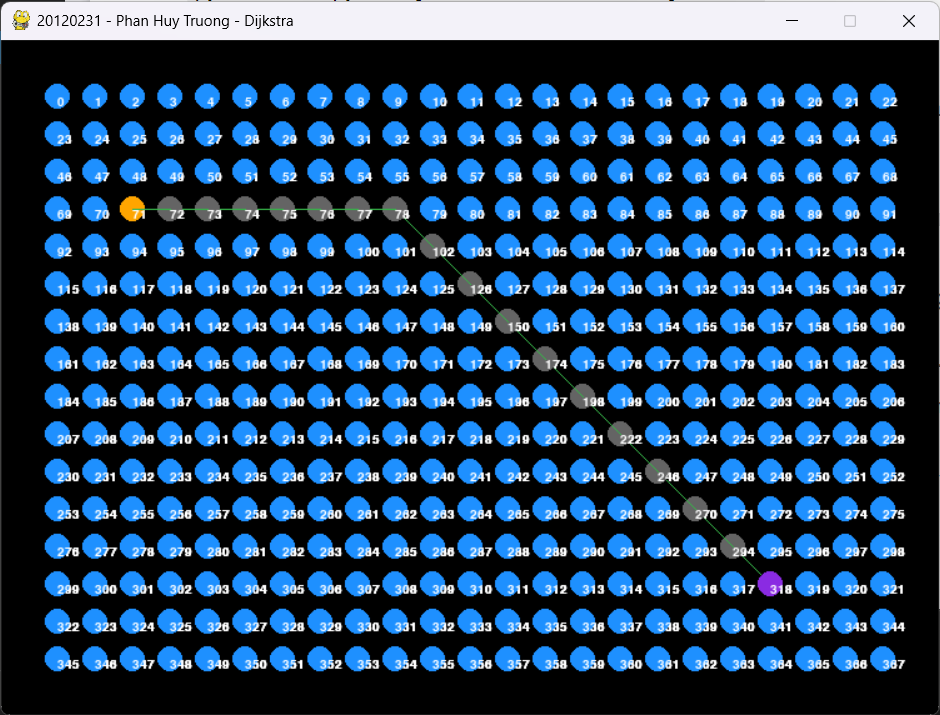
\includegraphics[width=4.5in, height=3in]{image/dijkstra_stimulation.png}}
    \vspace{2\baselineskip}
    \textbf{Mô tả: }
    \begin{itemize}
        \item Tư tưởng của thuật toán là tương tự UCS 
        \item Đầu tiên thuật toán khởi tạo danh sách có số lượng phần tử bằng số lượng các nút trong đồ thị. Mỗi phần tử tỏng danh sách có giá trị là vô cùng
        \item Trong quá trình thực hiện, thuật toán lưu lại chi phí của các nút vào danh sách $dist[]$ nếu chi phí tìm được là nhỏ hơn chi phí tại vị trí định danh được lưu trong danh sách và đưa vào danh sách closed\_set các nút đã được mở qua
        \item Đồng thời trong quá trình đó, chương trình cũng tiến hành lưu lại những nút cha để tiện cho việc vẽ lại đường đi
    \end{itemize}
    \textbf{Nhận xét: }
    \begin{itemize}
        \item Thuật toán trả về đường đi ngắn nhất từ một đỉnh đến tất cả đỉnh còn lại trong đồ thị
        \item Thuật toán cần nhiều thời gian hơn UCS do nó luôn tìm đường đi ngắn nhất đến tất cả các nút trước khi trả về đường đi tìm thấy
    \end{itemize}
\newpage

\begin{thebibliography}{5}
\bibitem{latex}\href{https://cloud.ducnn.com/s/QKNe9PmcBSdXF3g}{Stuart Russell and Peter Norvig, Artificial Intelligence: A Modern Approach, 4th Edition, Global Edition}

\bibitem{website} \href{https://gist.github.com/professormahi/cff4bfeaece05966e688658127bf41f3}{https://gist.github.com/professormahi/cff4bfeaece05966e688658127bf41f3}

\bibitem{1} \href{https://www.educative.io/answers/how-to-implement-a-breadth-first-search-in-python}{https://www.educative.io/answers/how-to-implement-a-breadth-first-search-in-python}

\bibitem{2} \href{https://www.geeksforgeeks.org/iterative-depth-first-traversal/
}{https://www.geeksforgeeks.org/iterative-depth-first-traversal/
}

\bibitem{3} \href{https://www.geeksforgeeks.org/python-program-for-dijkstras-shortest-path-algorithm-greedy-algo-7/
}{https://www.geeksforgeeks.org/python-program-for-dijkstras-shortest-path-algorithm-greedy-algo-7/
}

\bibitem{4} \href{https://www.hackerearth.com/practice/algorithms/graphs/depth-first-search/tutorial/
}{https://www.hackerearth.com/practice/algorithms/graphs/depth-first-search/tutorial/
}

\bibitem{5} \href{https://www.javatpoint.com/depth-first-search-algorithm
}{https://www.javatpoint.com/depth-first-search-algorithm
}

\bibitem{6} \href{https://gist.github.com/damienstanton/7de65065bf584a43f96a
}{https://gist.github.com/damienstanton/7de65065bf584a43f96a
}

\bibitem{7}
\href{https://www.geeksforgeeks.org/search-algorithms-in-ai/
}{https://www.geeksforgeeks.org/search-algorithms-in-ai/
}

\bibitem{8} 
\href{http://www.ccpo.odu.edu/~klinck/Reprints/PDF/wikipediaNav2018.pdf
}{http://www.ccpo.odu.edu/~klinck/Reprints/PDF/wikipediaNav2018.pdf
}

\bibitem{9}
\href{https://stackoverflow.com/questions/12806452/whats-the-difference-between-uniform-cost-search-and-dijkstras-algorithm
}{https://stackoverflow.com/questions/12806452/whats-the-difference-between-uniform-cost-search-and-dijkstras-algorithm
}

\end{thebibliography}
\end{document}

